\section{Methodology And Project Schedule}
\subsection{Project Methodology}
This project is fundamentally a design project and so the design will heavily depend on the system functional and non-functional requirements. These requirements will be verified through experimental analysis using both the mechanical and electrical engineering laboratories. Experimental analysis includes closed loop testing of the IoT system and power consumption of the Arduino carrier boards. The closed loop testing will provide experimental analysis to verify that the accelerometers, temperature sensors, ADC conversion, packet transmission and retrieval meet the design requirements of the system. Testing will also be conducted on the designed enclosure to ensure the system is sufficiently weather proof against heat and rain.  
\newpage
\subsection{Tasks and Schedule}

\begin{figure}[h!]
\center
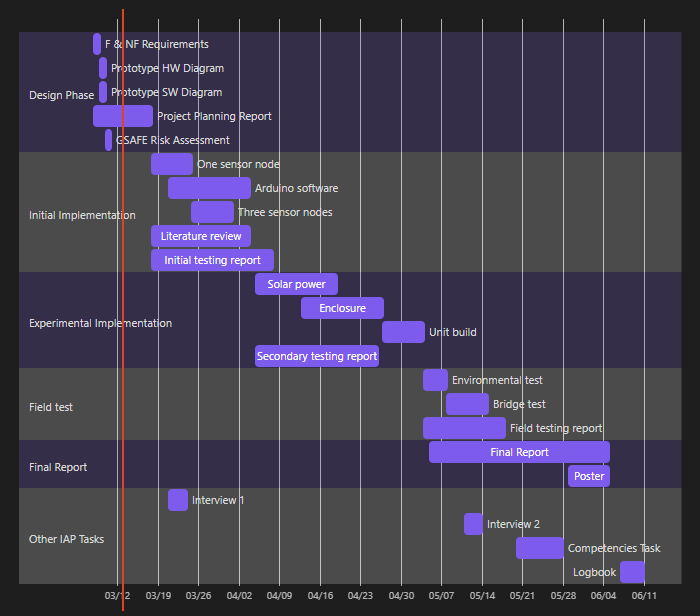
\includegraphics[scale=0.8]{Images/Gantt-Chart.png}
\caption{Project Timeline Gantt Chart}
\label{fig:GanttChart}
\end{figure}

\subsection{Resources}